\documentclass[12pt,a4paper]{ufpr}

\usepackage[brazil]{babel}
\usepackage[utf8]{inputenc}
\usepackage{amssymb,amsmath}
\usepackage{multirow}
\usepackage{amssymb}
\usepackage{subcaption}
\usepackage{graphicx}
\usepackage{caption}
\usepackage{setspace}
\usepackage{diagbox}

% n - numero de niveis de subsubsection numeradas
\setcounter{secnumdepth}{3}
% coloca ate o nivel n no sumario
\setcounter{tocdepth}{3}
\graphicspath{{img/}}

\title{WISYNC: SINCRONIZAÇÃO DE DIRETÓRIOS EM LAN}
\author{Renan Domingos Merlin Greca}
% ou Orientador
\advisortitle{Orientador}
\advisorname{Prof. Dr. Luiz Carlos P. Albini}
% departamento, instituicao
\advisorplace{Departamento de Informática, UFPR}
\city{Curitiba}
\year{2015}

% nao insira o nome do orientador, ja eh feito automaticamente
\banca{}{}{}{}{}{}{}{}

\defesa{X de janeiro de 2016}

\notaindicativa{Monografia apresentada para obtenção do Grau de
Bacharel em Ciência da Computação pela Universidade Federal do
Paraná.}

\begin{document}

\makecapa
\makerosto         % cria folha de rosto para versao final da UFPR %
%\maketermo      % cria folha com o termo de aprovacao da dissertacao%

%\singlespacing           % espacamento 1 - capa UFPR%
%\onehalfspacing          % espacamento 1/2 %
\doublespacing            % espacamento 2 - UFPR %

\pagestyle{headings}
\pagenumbering{roman}

%\chapter*{Agradecimentos}
%\input{agradecimentos.tex}          % possiu somente o texto

\tableofcontents

%\listoffigures         % se houver mais do que 3 figuras
%\addcontentsline{toc}{chapter}{\MakeUppercase{Lista de Figuras}}
%\newpage

%\listoftables        % se houver mais do que 3 tabelas
%\addcontentsline{toc}{chapter}{\MakeUppercase{Lista de Tabelas}}
%\newpage

% #################################################################################################

\chapter*{Resumo}
\addcontentsline{toc}{chapter}{\MakeUppercase{Resumo}}

[resumo]

\noindent \textbf{Palavras-chave}:

\chapter*{Abstract}
\addcontentsline{toc}{chapter}{\MakeUppercase{Abstract}}

[abstract]

\noindent \textbf{Keywords}:

\newpage

%\chapter*{Abstract}
%\addcontentsline{toc}{chapter}{\MakeUppercase{Abstract}}
%Texto do abstract....
        % somente o texto
%\newpage


\pagenumbering{arabic}

% #################################################################################################

\chapter{Introdução}
\label{introducao}
Com o barateamento e a popularização de microcomputadores, é comum hoje um escritório, uma família ou até mesmo um indivíduo ter diversos computadores pessoais à sua disposição.
Portanto, torna-se útil e às vezes necessário existir uma maneira de manter esses computadores ``conversando'' entre si, trocando informações e arquivos para que o usuário possa mudar de um para outro de forma coesa.
Além disso, computadores portáteis (i.e., \textit{laptops}) são mais vulneráveis do que computadores domésticos a roubos ou danos físicos, além de outros fatores que podem comprometer a integridade das informações neles contidas, o que torna necessária a realização de \textit{backups} frequentes.

Atualmente existem alguns programas disponíveis na Internet que fazem operações desse tipo, mas em contextos um pouco diferentes.

Entre produtos comerciais, há diversos serviços de armazenamento em nuvem\footnote{Com ``serviço em nuvem'', entende-se que o serviço funciona através de um servidor (ou um conjunto deles) na Internet; ou seja, os dados são armazenados em um servidor remoto ao usuário.\cite{mell2011nist}} que permitem que o usuário sincronize seus arquivos com um servidor na nuvem e com outros dispositivos, caso seja instalado um aplicativo em cada dispositivo. 
Exemplos desses produtos incluem Dropbox \cite{dropbox}, Box \cite{box}, Google Drive \cite{googledrive}, Apple iCloud Drive \cite{icloud} e Microsoft OneDrive \cite{onedrive}.
A principal diferença desses produtos ao atual projeto é a existência de um servidor mantendo os arquivos na nuvem.
A vantagem dessa decisão é que o usuário pode acessar seus arquivos facilmente de outros dispositivos como celulares e tablets \-- contudo, para a sincronização ocorrer é necessário que os computadores clientes estejam conectados à Internet e todos esses serviços impõem limites em bytes na quantidade de arquivos que podem ser sincronizados.

Outra categoria de programas que realizam operações semelhantes são os programas de \textit{backup}.
Um exemplo desses programas é o FreeFileSync \cite{freefilesync}, solução \textit{open-source} disponível na web.
Dados um par de diretórios A e B, programas de \textit{backup} normalmente possuem três funcionalidades:
\begin{itemize}
    \item Sincronização de dois sentidos, que torna A e B idênticos copiando as modificações de um para o outro e vice-versa;
    \item Sincronização de espelho, que faz o diretório B ser um clone do diretório A, incluindo arquivos removidos; e
    \item Sincronização de atualização, que atualiza B com os arquivos novos ou modificados de A, mas não remove arquivos excluídos em A.
\end{itemize}

Para o propósito desta monografia, o projeto irá focar no primeiro tipo de sincronização, a de dois sentidos.
Os outros dois tipos também são interessantes e possivelmente serão adicionados ao escopo futuramente.

Enquanto o FreeFileSync sincroniza dois diretórios no mesmo computador e os serviços em nuvem se beneficiam de um servidor remoto que gerencia a sincronização, o objetivo deste projeto é desenvolver um programa que funcione de maneira local, ou seja, fazendo dois computadores interagirem pela rede sem um servidor no meio.
Comparado às soluções em nuvem, isso permite que o programa seja rodado sem uma conexão à Internet, não impõe limites de dados e também resulta numa velocidade maior na transferência dos arquivos.
Contudo, requer que ambos computadores estejam conectados à mesma rede e torna a sincronização em si um pouco mais complicada.

Programas que dependem da comunicação em rede são naturalmente desafiadores, pois eles dependem muito de fatores externos para funcionarem como esperado.
No caso deste projeto, duas instâncias do programa estarão rodando simultaneamente numa rede e devem se encontrar e se comunicar.
Então, além do desafio natural de comparar diretórios e transferir arquivos pela rede local, deve-se sempre manter em mente a sinergia entre as duas instâncias do programa, garantindo que uma esteja sempre preparada para a próxima ação da outra.

\section{Proposta}
Para trabalhar em diversos computadores ou manter cópias seguras de arquivos de forma conveniente, o presente projeto propõe um programa que, através de uma rede local (daqui em diante referida como LAN, de \textit{Local Area Network}), compare diretórios em dois ou mais computadores distintos e realize a sincronização dos mesmos.
Com sincronização, queremos dizer que o programa irá, para cada instância rodando:
\begin{itemize}
    \item Copiar arquivos novos (adicionados desde a última execução) às outras instâncias;
    \item Apagar arquivos removidos nas outras instâncias; e
    \item Copiar alterações aos arquivos às outras instâncias, incluindo arquivos renomeados.
\end{itemize}

% #################################################################################################

\chapter{Revisão Bibliográfica}
\label{revisao}

\section{Python}

Python\cite{python} é uma das linguagens de programação de alto nível mais populares no momento em que este texto foi escrito\cite{toplanguages2015}. Isso se deve em parte à facilidade em aprendê-la, à agilidade ao escrever software, à ampla disponibilidade de bibliotecas eficientes e à grande comunidade disposta a auxiliar outros programadores. 
É uma linguagem interpretada, então programas criados com ela não enfatizam desempenho, sendo frequentemente muitas vezes mais lentos do que programas similares construídos em linguagens como C ou Java[falta referência].
Contudo, essa lentidão só se demonstra um problema em algoritmos computacionalmente pesados.
Quando esse não é o caso, um programador pode optar pelo desenvolvimento mais rápido do Python em troca de alguns segundos a mais na hora de rodar o programa.

\section{Sobre a Transmissão dos Arquivos}
A primeira etapa do desenvolvimento do programa foi definir o método e protocolo que seriam usados na hora de transmitir arquivos entre os computadores.
Após alguma pesquisa, quatro alternativas foram consideradas: 
\begin{itemize}
  \item \textbf{Sockets via TCP}, que utilizaria a biblioteca padrão \texttt{socket} do Python\cite{pythonsockets} para transmitir os dados dos arquivos a nível de camada de transporte utilizando o TCP (Transmission Control Protocol). A implementação em Python é relativamente simples, mas requer muita atenção porque arquivos maiores têm que ser divididos em blocos para depois serem re-montados. O TCP cuida da confiabilidade da transmissão dos blocos de arquivo\cite{cerf2005protocol}, mas o programador tem que se preocupar com a organização desses blocos quando recebidos.
  \item \textbf{Secure Copy} (SCP), método que utiliza os mesmos padrões de segurança do protocolo SSH (\textit{secure shell}) para garantir a segurança e confidencialidade dos dados\cite{scpcommand}. A maneira mais simples de fazer isso em Python seria invocando um comando da linha de comando, que não dá muito controle sobre a operação de dentro do programa.
  \item \textbf{File Transfer Protocol} (FTP) é um protocolo da camada de aplicação específico para o envio de arquivos. Na sua especificação, entre seus objetivos constam ``1) promover o compartilhamento de arquivos, 2) encorajar uso de computadores remotos, 3) proteger o usuário de variões de sistemas de arquivos e 4) transferir dados de forma confiável e eficiente''\cite{rfc959}. Contudo, ele se mostra mais eficaz em situações onde há servidor e clientes bem definidos: ou seja, um servidor que hospeda arquivos e clientes que podem acessar e alterar os arquivos do servidor.
  \item \textbf{Hypertext Transfer Protocol} (HTTP) é o protocolo padrão de envio de dados na Internet, cuja versão 1.1, definida em 1997 e atualizada em 1999\cite{rfc2616}, é atualmente utilizada[falta referência]. É fácil de utilizar, mas seu principal objetivo não é o envio de arquivos. Como é o protocolo padrão da Internet, é possível acessar os arquivos por um navegador se o endereço for conhecido.
\end{itemize}

\section {JSON}
O \textit{JavaScript Object Notation}, ou JSON, é um formato de armazenamento e troca de dados baseado na notação de objetos do JavaScript. Com o JSON, é possível armazenar objetos de um programa em um arquivo de texto, utilizando os tipos \textit{array}, \textit{string}, \textit{number} e \textit{boolean} do JavaScript\cite{json}.
O JSON foi escolhido por sua simples integração com Python e por ser um formato facilmente legível por um humano, facilitando a verificação dos dados durante os testes.
Contudo, essa facilidade de leitura também se mostra um risco, já que é possível alterar os dados armazenados por fora do programa e então gerar resultados inesperados.

% #################################################################################################

\chapter{Desenvolvimento}
\label{desenvolvimento}
Neste capítulo, será descrita o desenvolvimento e as soluções da implementação do WiSync para este trabalho.

A versão do WiSync entregue com este texto foi escrita em Python \cite{python}, versão 2.7.
Python foi escolhida por sua facilidade na implementação e extensa disponibilidade de bibliotecas de código aberto.

Originalmente, havia como objetivo tornar o programa compatível com os três sistemas operacionais mais comuns do mundo: Microsoft Windows, Apple OS X e Linux.
Contudo, devido a diferenças inerentes na forma como o Windows funciona, optou-se por manter apenas compatibilidade com OS X e Linux.
Para tal, o WiSync foi desenvolvido usando os seguintes computadores para testes:

\begin{center}
  \begin{tabular}{ l | l | l }
    \hline
    \textbf{Nome} & ``SgtPepper'' & ``Packard'' \\ \hline \hline
    Sistema Operacional & OS X 10.11 & Linux Mint 17 \\ \hline
    Processador & Intel Core i5-4308U & Intel Core i7-2600 \\ \hline
    RAM & 8GB DDR3L & 8GB DDR3 \\ \hline
    Armazenamento & SSD 512GB & HDD 320GB \\ \hline
    Conectividade & Wi-Fi 802.11n 5GHz & Cabo Ethernet \\ \hline
    IP local & 192.168.1.110 & 192.168.1.132 \\
    \hline
  \end{tabular}
\end{center}

\section{Bibliotecas Usadas}
Para executar o WiSync, são necessárias algumas bibliotecas padrão do Python: \texttt{os}, \texttt{sys}, \texttt{argparse}, \texttt{time}, \texttt{json}, \texttt{datetime}.
Também é usada uma versão modificada do programa \texttt{woof.py} \cite{woof} (distribuída sob a licença GNU General Public License), que é usada na hora de transmitir os arquivos entre os computadores.
No WiSync, arquivos JSON são usados para armazenar e transmitir as listas de arquivos geradas pela leitura e comparação dos diretórios.

O HTTP foi escolhido para realizar a troca de arquivos do WiSync.
Isso se deve principalmente à facilidade de implementar essa troca, e também ao fato que dois computadores podem rapidamente trocar seus papéis de cliente e servidor enquanto transmitem arquivos entre si.
Como o objetivo do WiSync é ser usado em redes locais privadas, a abertura temporária dos arquivos na rede não é uma grande preocupação.

\subsection{Mudanças feitas ao woof}
Como citado anteriormente, o programa \texttt{woof.py} \cite{woof} foi usado como biblioteca para auxiliar no envio de arquivos por HTTP.
Para se adequar às necessidades do WiSync, algumas pequenas mas importantes mudanças tiveram que ser feitas:
\begin{itemize}
  \item Após servir um arquivo ao outro computador, o endereço IP do computador remoto é armazenado para poder ser utilizado novamente no futuro sem depender de outras buscas por endereços.
  \item Originalmente, o \texttt{woof.py} utilizava diversas \textit{threads} para permitir o \textit{download} simultâneo de arquivos. Como essa funcionalidade não é necessária para o WiSync e as múltiplas \textit{threads} causavam consequências indesejadas, o código foi alterado para desabilitar isso.
\end{itemize}

\section{Situações consideradas}
Tratando-se das possíveis diferenças que podem existir entre um par de diretórios (vamos chamá-los de A e B), as seguintes possibilidades são consideradas:
\begin{itemize}
  \item Arquivos existem em A mas não em B e vice-versa. Como demonstrado na figura \ref{a}, nessa situação basta copiar os arquivos do diretório que os contém para o que não os contém.
  \begin{figure}[h]
    \centering
    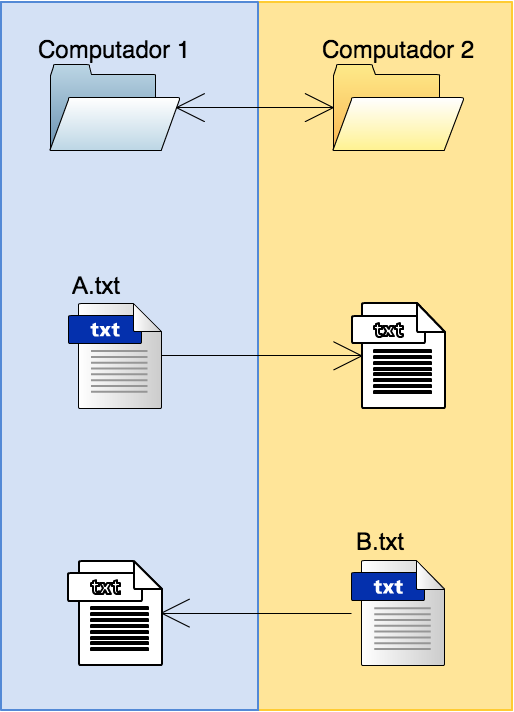
\includegraphics[width=200pt]{img/a.png}
    \caption{Caso onde os dois diretórios têm arquivos novos}
    \label{a}
  \end{figure}
  \item Arquivos com o mesmo nome existem em A e B mas têm conteúdo diferentes. Caso da figura \ref{b}. Nesse caso o WiSync utiliza o histórico da última sincronização antes da atual e as informações de data de modificação dos arquivos. Se o arquivo já existia antes e a data de alteração de uma das versões atuais é igual à anterior (implicando que o arquivo não foi modificado desde então), a versão mais recente substitui a mais antiga. O mesmo processo se aplica a um arquivo que foi excluído desde a última sincronização.
  \begin{figure}[h]
    \centering
    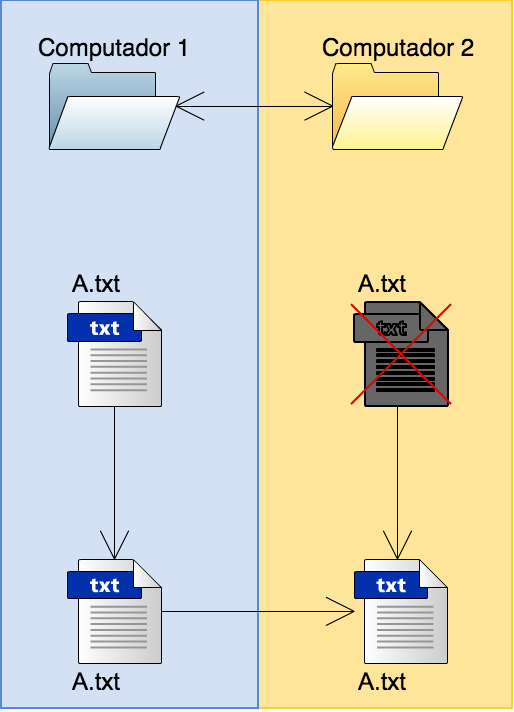
\includegraphics[width=200pt]{img/b.png}
    \caption{Caso onde um arquivo foi atualizado em apenas um dos diretórios}
    \label{b}
  \end{figure}
  \item Similar à situação acima, mas ambos arquivos têm datas de modificação diferentes às da última sincronização, ou não há informação sobre a última sincronização. Nesse caso, mostrado na figura \ref{c}, o WiSync copia ambas versões para o outro diretório, renomeando os arquivos para evitar conflitos e sobre-escritas.
  \begin{figure}[h]
    \centering
    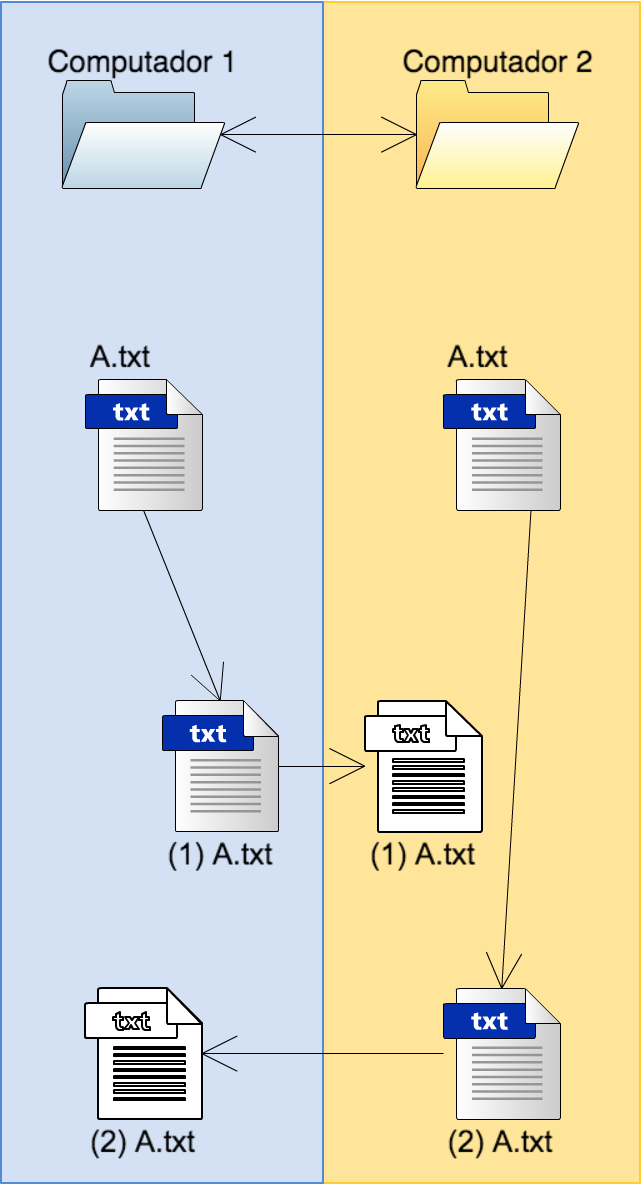
\includegraphics[width=200pt]{img/c.png}
    \caption{Caso onde há conflito de versões entre dois arquivos}
    \label{c}
  \end{figure}
  \item Caso um arquivo seja renomeado, o WiSync tratará essa situação como se fossem dois arquivos: um excluído e um novo. Caso o arquivo correspondente no diretório remoto não tenha sido alterado desde a última sincronização, este será excluído e uma nova cópia, com o novo nome, será criada. Isso é ilustrado na figura \ref{d}
  \begin{figure}[h]
    \centering
    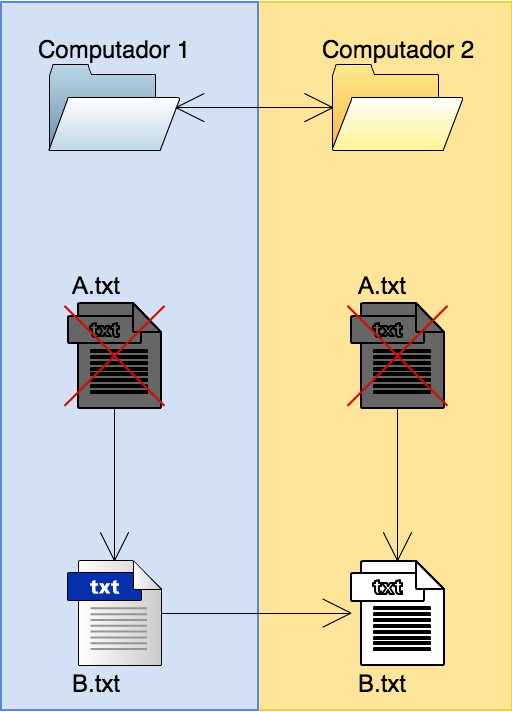
\includegraphics[width=200pt]{img/d.png}
    \caption{Caso onde um arquivo foi renomeado}
    \label{d}
  \end{figure}
\end{itemize}

\section{Fluxo do programa}
Durante a execução, o WiSync executa as seguintes operações:
\begin{enumerate}
  \item Processa parâmetros e configura as classes WiFiles e WiNet, que preparam o que é necessário para lidar com arquivos e rede no programa.
    \item As duas instâncias do programa trocam os arquivos JSON contendo informações sobre o diretório a ser sincronizado.
    \item Uma das instâncias utiliza esses arquivos JSON e, se existir, o arquivo contendo informações do estado anterior do diretório para gerar um novo JSON contendo a lista de arquivos que devem ser transferidos ou excluídos em cada um dos diretórios.
    \item A instância que realizou a comparação começa a enviar os arquivos de acordo com a lista contida no JSON e, ao mesmo tempo, a outra instância recebe esses arquivos.
    \item As instâncias trocam e a segunda passa a enviar arquivos para a primeira.
    \item Ambas instâncias excluem seus próprios arquivos de acordo com o JSON.
    \item Um novo JSON é gerado contendo as informações dos diretórios após a sincronização, que será usado para sincronizações futuras.
\end{enumerate}

\section{Dificuldades encontradas}
Durante o desenvolvimento do WiSync, algumas dificuldades foram encontradas.
A seguir elas são descritas e são apresentadas as soluções encontradas.

\subsection{Waits e timeouts}
Talvez a parte mais difícil do desenvolvimento do WiSync tenha sido levar em consideração o fato de que o programa roda em dois computadores diferentes, com velocidades diferentes e que se comunicam apenas ocasionalmente através da troca de arquivos.
Para evitar erros, é necessário garantir que ambos computadores estejam no mesmo passo ao mesmo tempo.

Um erro que aconteceu com frequência durante o desenvolvimento, por exemplo, é que um computador procurava o arquivo do outro antes deste ter preparado a hospedagem do arquivo.
Ou seja, o arquivo não estava disponível ainda e o primeiro computador retornava um erro de endereço inválido.
Para evitar isso, foi adicionado uma pausa de 1 segundo logo antes de tentar acessar um arquivo do outro computador.
Este tempo permite que o outro computador termine de preparar a hospedagem.
Essa solução não é infalível, pois pode ser que o computador demore mais ainda para hospedar e, neste caso, o erro acontece de qualquer forma.
Uma solução para isso seria criar um laço onde se tenta diversas vezes acessar o arquivo remoto mas, nos testes, isso teve um desempenho pior do que a pausa.

\subsection{Datas de criação/modificação}
Como explicado anteriormente, o WiSync utiliza metadados dos arquivos \-- a data modificação em particular \-- para decidir quais devem ser copiados.
Contudo, isso gerou um problema que não havia sido previsto: quando um arquivo é copiado para o outro, a data de modificação da cópia é a data de sincronização \-- não a data de modificação do arquivo original.
Ou seja, numa sincronização subsequente, a cópia é entendida como uma versão nova do arquivo e copiada novamente para o computador original.

Para resolver isso, foi usada a função \texttt{os.utime} do Python, dessa forma configurando as datas de criação e modificação do arquivo criado para serem iguais às do arquivo de origem. Uma preocupação que surgiu em relação a isso foi a possibilidade de, devido a configurações diferentes entre os computadores, um arquivo ter data de criação e/ou modificação futura ao relógio do sistema.
Contudo, testes foram realizados no Linux e no OS X e isso não se mostrou um problema.

\subsection{Ordem dos arquivos}
As listas de arquivos que o WiSync são armazenadas usando o tipo Dictionary, do Python, para que torne-se simples indexar os arquivos utilizando os nomes deles.
Contudo, um dicionário, ao ser percorrido, não tem uma sequência definida a ser seguida. 
ortanto, na hora de enviar e receber arquivos, o dicionário é convertido para uma lista de tuplas, ordenada alfabeticamente com os nomes dos arquivos.
Isso garante que ambos computadores enviem e recebam arquivos na mesma ordem.

% #################################################################################################

\chapter{Resultados}
\label{resultados}

\section{Organização do Programa}
O WiSync é composto por três arquivos: \texttt{wisync.py}, \texttt{winet.py} e \texttt{wifiles.py}. Abaixo estão as funcionalidades de cada um:
\begin{itemize}
  \item \texttt{wisync.py}: Arquivo principal do projeto, responsável por ler os parâmetros da linha de comando e controlar a execução do processo.
  \item \texttt{winet.py}: Contém a classe WiNet, que inclui os métodos e atributos necessários para fazer as partes em rede do programa, como hospedar e receber arquivos.
  \item \texttt{wifiles.py}: Contém a classe WiFiles, que inclui os métodos e atributos necessários fazer as partes que lidam com o sistema de arquivos do programa, como ler e comparar diretórios.
\end{itemize}

\subsection{Parâmetros de Execução}

Para rodar o WiSync, utiliza-se o seguinte comando:
\begin{verbatim}
python wisync.py [-h] -d DIRECTORY [-n HOSTNAME] [-s]
\end{verbatim}

Os argumentos são os seguintes:
\begin{itemize}
  \item \texttt{-h, --help} Mostra o texto de ajuda do programa.
  \item \texttt{-d DIRECTORY, --directory DIRECTORY} Caminho para o diretório a ser sincronizado (de preferência, o caminho completo)
  \item \texttt{-n HOSTNAME, --hostname HOSTNAME} Nome de rede ou endereço IP do outro computador. Esse argumento é opcional e pode ser preenchido tanto pelo endereço IP do outro computador quanto pelo nome de rede. Por exemplo, \texttt{-n SgtPepper.local} e \texttt{-n 192.168.1.110} têm o mesmo efeito. Caso o argumento não esteja presente, o programa procura outras instâncias do WiSync na rede local.
  \item \texttt{-s, --server} Modo servidor. Se definido, esta instância será o ``servidor'', hospedando seus arquivos antes da instância remota.
\end{itemize}

% #################################################################################################

\chapter{Conclusão}
\label{conclusao}

[conclusão]

% Trocar para ficar no padrão brasileiro
%\bibliographystyle{brazil}
\bibliographystyle{brazil}
\bibliography{bib}
% utilize macros (3 primeiras letras do mes em ingles, minusculas) no seu
% .bib para atribuir o nome do mes em portugues nas referencia,
% se o style for brazil, outros estilos tambem aceitam estas macros
% Ex:
%
% @InProceedings{teste,
%   author =       {Luciano}
%   year =         {2000}
%   month =        {}#sep;
% }
%
\addcontentsline{toc}{chapter}{\MakeUppercase{Bibliografia}}

\singlespacing

\end{document}
